\documentclass[t]{beamer}


\newcommand{\coursename}{CVX-BigData}
\newcommand{\lecturenumber}{5}
\newcommand{\vx}{\ensuremath{\mathsf{x}}}
\newcommand{\vparam}{\ensuremath{\theta}}
\newcommand{\param}{\ensuremath{\theta_{\alpha}}}
\newcommand{\vmean}{\ensuremath{\mu}}
\newcommand{\mean}{\ensuremath{\mu_{\alpha}}}
\newcommand{\vsuff}{\ensuremath{\phi}}
\newcommand{\suff}{\ensuremath{\phi_{\alpha}}}

\newcommand{\set}[1]{\ensuremath{\left\{ #1 \right\}}}

\date[July 2017] {July 2017}
\title{Graphical Model and Connection to Convex Optimization}
\author{Han Xiao, Sijing Tu}
\institute[] % (optional, but mostly needed)
{
  Department of Computer Science\\
  Aalto University
}

\newcommand{\leftMargin}{8ex}

\beamertemplatenavigationsymbolsempty
\setbeamertemplate{headline}{%
\ifnum \value{framenumber}=1
\leavevmode%
  \hbox{%
    \begin{beamercolorbox}[wd=.5\paperwidth,ht=2.8em,dp=2ex,left]{normal text}%
      \usebeamerfont{author in head/foot}
      \hspace*{\leftMargin}   \insertauthor
    \end{beamercolorbox}%
    \begin{beamercolorbox}[wd=.5\paperwidth,ht=2.8em,dp=2ex,right]{normal text}%
      \usebeamerfont{date in head/foot}
      \coursename \hspace*{\leftMargin} 
    \end{beamercolorbox}}%
    \vskip0pt%
    \else
      \fi
}
\defbeamertemplate*{title page}{customized}[1][]
{
	\vspace*{2ex}
  	{\centering \usebeamerfont{title} \textbf{\lecturenumber. \inserttitle}\par}
	\vspace*{1cm}

  	\begin{minipage}[c][1.8cm][c]{\textwidth}
	\tableofcontents[currentsection]
	\end{minipage}

}
\setbeamertemplate{frametitle}
{
    \nointerlineskip
    \begin{beamercolorbox}[sep=0.3cm,ht=2.5em,wd=\paperwidth,center]{frametitle}
        \textbf{\insertframetitle}
    \end{beamercolorbox}
}
\defbeamertemplate*{footline}{nooutlinefooter}
{
  \leavevmode%
  \hbox{%
  
  \begin{beamercolorbox}[wd=.5\paperwidth,ht=2.8em,dp=2ex,left]{normal text}%
    \usebeamerfont{title in head/foot}
    \vspace*{4ex} \hspace*{\leftMargin}  
    \ifnum \value{framenumber}>1
	    \insertshorttitle
    \fi
  \end{beamercolorbox}%

  \begin{beamercolorbox}[wd=.5\paperwidth,ht=2.8em,dp=2ex,right]{normal text}%
    \usebeamerfont{date in head/foot} \vspace*{4ex}
    \lecturenumber-\insertframenumber{} \hspace*{\leftMargin} 
  \end{beamercolorbox}}%
  \vskip0pt%
}

\setbeamertemplate{nooutlinefooter}


\setbeamertemplate{itemize item}[circle]
\setbeamercolor{itemize item}{fg=black}

\setbeamercolor{frametitle}{fg=black}
\setbeamercolor{normal text}{fg=black,bg=white}

\setbeamertemplate{section in toc}[ball unnumbered]
\setbeamercolor{section in toc}{fg=black,bg=black}
\setbeamertemplate{section in toc shaded}[default][100]
\setbeamerfont{section in toc shaded}{series=\mdseries}
\setbeamerfont{section in toc}{series=\bfseries}

\setbeamercolor{item projected}{bg=black,fg=black}
\AtBeginSection[]
{
  \ifnum \value{framenumber}>1
    \begin{frame}[plain, noframenumbering]
    	\frametitle{Outline}
		\vspace*{1cm}
	  	\begin{minipage}[c][1.8cm][c]{\textwidth}
			\tableofcontents[currentsection]
		\end{minipage}
    \end{frame}
  \else
  \fi
}
\setbeamersize{text margin left=4ex}
\setbeamersize{text margin right=4ex}

% Let's get started
\begin{document}
\maketitle

\begin{frame}{What you will learn today}
   \begin{itemize}
   \setlength\itemsep{0.5em}
   \item {Graphical model
   \begin{itemize}
     \item Basic concepts 
     \item Special case -- exponential family
     \end{itemize}
   }
   \item Properties of exponential family 
   \item Connection to convex optimization
   \end{itemize}
\end{frame}

\section{Graphical Models and Exponential Family}
\begin{frame}{Motivation}
   \begin{itemize}
	\item {main idea: reduce parameter space by bringing in "structure" to the model
    	\begin{itemize}
	    \item without any structure, $O(2^N)$ parameters to specify a model of $N$ random binary variables
    	\item with proper structures, parameter space can be reduced to polynomial
    	\end{itemize}}
    \item based on correspondence between \textit{graphs} (therefore called ``graphical models'') and random variables
    \item \textit{exponential family} contains a variety of such models.
   \end{itemize}
\end{frame}

\newcommand{\suffset}{\ensuremath{\mathcal{I}}}
\newcommand{\real}{\ensuremath{\mathcal{R}}}
\newcommand{\measure}{\ensuremath{\mathit{v}}}
\newcommand{\innerprod}[1]{\ensuremath{\langle #1 \rangle}}
\newcommand{\pp}{\ensuremath{p_{\vparam}}}

\begin{frame}{Exponential family}
   \begin{itemize}
	\item parametric family of density function: $\pp(\vx) = \exp \set{\sum\limits_{\alpha} \param \suff (\vx) - A(\vparam) }$
	   		\item $\suff: X^n \rightarrow \real$, sufficient statistics
        	\item $\vsuff = \set{\suff, \alpha \in \suffset}$, set of sufficient statistics
        	\item $\vparam = \set{\param, \alpha \in \suffset}$, canonical parameters
        	\item $\suffset$ defined by graph topology $G=(V, E)$ (example shown later)
   \end{itemize}
\end{frame}

\begin{frame}{Exponential family: continued}
   \begin{itemize}
	\item {cumulant generating function (log normalization constant) 
   	$A(\vparam) = \log \left( \int \exp \{ \innerprod{\vparam, \vsuff(\vx)} \measure (d \vx) \} \right)$
	   \begin{itemize}
	   		\item {$\innerprod{\ldots}$: vector dot product}
	   		\item {$\measure$: base measure}	   		
	   \end{itemize}	   		
	}
	\item $A(\vparam)$ is convex
   \end{itemize}
\end{frame}

\begin{frame}{Example: Ising model}
	\begin{itemize}
		\item $\pp(\vx) = \exp \set{\sum\limits_{s \in V} \theta_s x_s + \sum\limits_{(s, t) \in E} \theta_{st} x_s x_t  - A(\theta) }$
		\item $x_s \in \set{0, 1} \text{ for all } s \in V$ (discrete and binary)
		\item {$V$ and $E$: random variables (nodes) and  pairwise relationship (edges) respectively
			\begin{figure}
				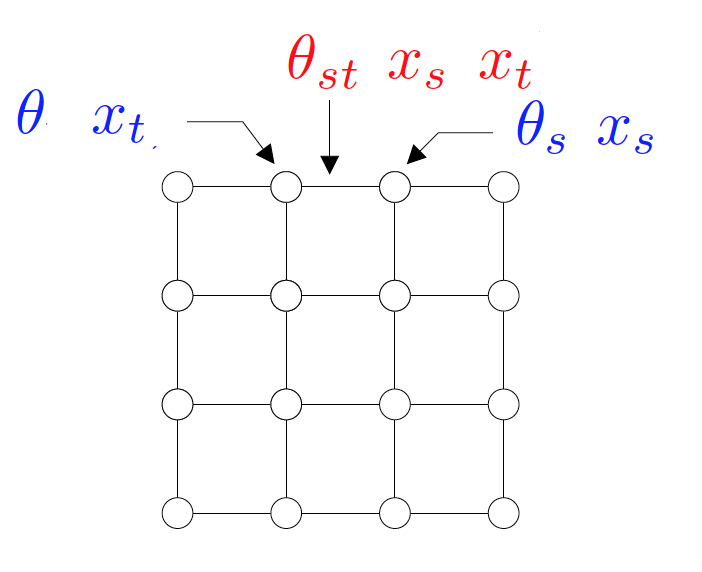
\includegraphics[width=0.3\textwidth]{ising}
			\end{figure}
		}
		\item number of parameters $\approx 5N = O(N) \ll O(2^N) $ (reduced a lot!)
	\end{itemize}
\end{frame}

\begin{frame}{Example: Gaussian Markov Random Field (GMRF)}
	\begin{itemize}
		\item $\pp(\vx) = \exp \set{ \innerprod{\vparam, \vx} + \frac{1}{2} \langle\langle \Theta, \vx \vx^T \rangle\rangle - A(\theta) }$
		\item $\vx=\set{x_1, \ldots, x_N}$ follows multivariate Gaussian distribution
		\item $\langle\langle \Theta, \vx \vx^T \rangle\rangle = \text{trace}(\Theta \vx \vx^T)  = \sum\limits_{i=1}^N \sum\limits_{j=1}^N \Theta_{ij} \vx_i\vx_j $
    	\item number of parameters $N + N^2 = O(N^2) \ll O(2^N)$ (reduced a lot!)
	\end{itemize}
\end{frame}

% \newcommand{\sup}{\ensuremath{\text{sup}}

\section{Properties of Exponential Family}

\begin{frame}{Alternative representation via mean parameters}
	\begin{itemize}
		\item any exponential family can be represented alternatively by some mean parameters $
		\vmean$ (w.r.t canonical parameters $\vparam$)
		\item definition $\mean = \int  \suff(\vx) p(\vx) \measure(d \vx) $ for all $\alpha \in \suffset$
		\item {example mean parameters:
		\begin{itemize}		
			\item Ising : $\mu_s=\text{Pr}[X_s=1]$ and $\mu_{st}=\text{Pr}[(X_{s}, X_{t})=(1, 1)] $
			\item GMRF: $\mu=\mathbb{E}[X]$ and $\Sigma=\mathbb{E}[XX^T]$
		\end{itemize}			
		}
		\item {$\vmean$ is characterized by conjugate convex function: 
		\begin{equation}
			\label{conjugate}
			A^{*}(\vmean) = \sup_{\vparam} (\innerprod{\vmean, \vparam} - A(\vparam))
		\end{equation}
		}	
	\end{itemize}
\end{frame}

\begin{frame}{Theorems (adapted from theorem 3.4 in \cite{main})}
\begin{enumerate}
	\item {for any $\vparam$, supremum in Equation~\ref{conjugate} is achieved \textit{uniquely} by \textit{moment matching condition (denote such $\mu$ by $\mu(\theta)$)} 
	\[\mu = \int  \vsuff(\vx) \pp(\vx) \measure(d \vx)\]}
	\item {for any \textit{realizable} $\vmean$, 
	\[A^{*}(\vmean) = -H(p_{\mu(\theta)}) \quad \text{(negative entropy)}\]
	}
	\item {$A(\vparam)$ has variational representation
	\begin{equation}
		\label{variational}
		A(\vparam) = \sup_{\vmean} (\innerprod{\vparam, \vmean} - A^{*}(\vmean))
	\end{equation}
	}
\end{enumerate}
\end{frame}

\begin{frame}{Why are they important?}
	\begin{enumerate}
		\item implies the bijection nature between canonical parameter space ($\set{\theta}$) and mean parameter space ($\set{\mu}$)
		\item {states the duality between $A$ and entropy 
			\begin{itemize}
				\item $A^{*}(\mu)$ is the optimum of the maximum entropy problem in (Problem 3.3 in \cite{main})
			\end{itemize}
		}
		\item {computing $A(\vparam)$ is fundamental for important inference problems such as computing marginal distribution
			\begin{itemize}
				\item computing $A(\vparam)$ becomes a \textbf{optimization problem} via variational representation (Equation~\ref{variational})
			\end{itemize}
		}
		\item {$A(\theta)$ and $\mu$ are computed simultaneously}		
	\end{enumerate}
\end{frame}

\section{Connection to Convex Optimization: Examples}

\begin{frame}{Ising model: marginal probability}
	\begin{itemize}
		\item problem: given $\theta$, compute $\text{Pr}[X_s=1]$ for some $s \in V$
		\item actually a mean parameter $\mu_s=\text{Pr}[X_s=1]$
		\item {therefore equivalent to solve $\text{argmax}_\mu \set{\theta^T \mu - A^{*}(\mu) } $
			\begin{itemize}
				\item a convex optimization problem!
			\end{itemize}
		}
		\item $\mu$ and $A(\theta)$ is computed simultaneously!		
	\end{itemize}
\end{frame}

\begin{frame}{GMRF: $\mu$ under fixed covariance}
	\begin{itemize}
		\item problem: given covariance $Q$ and canonical parameter $\vparam$, compute the corresponding $\mu$ (because of bijection relationship)
		\item {straightforward computation  based on $A(\theta) $leads to
			\[ A^{*}(\mu) = \frac{1}{2} \mu^T Q \mu + \text{constant} \]
		}
		\item {variational representation (\textbf{maximization problem!})
			 \[ A(\theta) = \sup_{\mu} \set{\theta^T \mu - \frac{1}{2} \mu^T Q \mu } + \text{constant} \]
		 }
		\item {optimum achieved uniquely at $\mu = Q^{-1} \theta$ (because of convexity)
			\begin{itemize}
				\item can be calculated by fixed point method
			\end{itemize}
		}
	\end{itemize}		
\end{frame}

\begin{frame}{What you have learned today}
	\begin{itemize}
		\item why using graphical models -- reduce parameter space
		\item {exponential family and its properties:
			\begin{itemize}		
			\item bijection between canonical parameter $\set{\theta}$ and mean parameter $\set{\mu}$ for such family
			\item variational representation of $A(\theta)$
			\item calculating $A(\theta)$ and obtaining optimal $\mu$ are done simultaneously
			\end{itemize}			
		}
		\item two exponential family examples and how convex optimization connects to them specifically
	\end{itemize}
\end{frame}

\begin{thebibliography}{9}

\bibitem{main}
Wainwright, M. J., \& Jordan, M. I. (2008). 
Graphical models, exponential families, and variational inference. 
\textit{Foundations and Trends® in Machine Learning}, 
1(1–2), 1-305.
\end{thebibliography}

\end{document}


